\documentclass[conference]{IEEEtran}
\usepackage{cite}
\usepackage{amsmath,amssymb,amsfonts}
\usepackage{graphicx}
\usepackage{textcomp}
\usepackage{xcolor}
\usepackage{booktabs}
\usepackage{multirow}

\begin{document}

\title{Network-Based Analysis of Polymer-Clay Nanocomposite Mechanical Properties: A Modulus-Driven Clustering Approach}

\author{\IEEEauthorblockN{1\textsuperscript{st} Berfin Dolunay Karaçay}
\IEEEauthorblockA{\textit{Department of Computer Engineering} \\
\textit{TED University)}\\
Ankara, Türkiye \\
bdolunay.karacay@tedu.edu.tr}
\and
\IEEEauthorblockN{2\textsuperscript{nd} Selin Siviş}
\IEEEauthorblockA{\textit{Department of Computer Engineering)} \\
\textit{TED University}\\
Ankara, Türkiye \\
selin.sivis@tedu.edu.tr}
\and
\IEEEauthorblockN{3\textsuperscript{rd} Gökçe Nur Yılmaz}
\IEEEauthorblockA{\textit{Department of Computer Engineering} \\
\textit{TED University)}\\
Ankara, Türkiye \\
gokce.yilmaz@tedu.edu.tr}
\and
\IEEEauthorblockN{4\textsuperscript{th} Ayşe Çağıl Kandemir}
\IEEEauthorblockA{\textit{Department of Mechanical Engineering} \\
\textit{TED University}\\
Ankara, Türkiye \\
cagil.kandemir@tedu.edu.tr}

}

\maketitle

\begin{abstract}
This study presents a novel graph-theoretic approach for analyzing the mechanical property enhancement patterns in polymer-clay nanocomposites \cite{112, 127}. A comprehensive dataset of 927 nanocomposite samples extracted from 148 peer-reviewed publications \cite{1}-\cite{148} was systematically organized into four clusters based on neat polymer matrix elastic modulus, ranging from soft elastomeric systems (0-0.1 GPa) to rigid polymer matrices (>1.0 GPa). Bipartite graphs were constructed for each cluster to represent relationships between polymer matrices and their corresponding nanocomposite formulations, with edge weights quantifying elastic modulus improvements \cite{10, 11}. Centrality metrics including degree, weighted degree, and betweenness centrality were computed to identify ``knowledge hubs'' representing polymer systems with substantial cumulative property improvements. Results reveal an inverse relationship between matrix stiffness and improvement magnitude, with soft elastomeric systems achieving 288-351\% average improvements compared to 33-46\% for rigid polymers \cite{14, 22}. Surface modification effectiveness was found to be stiffness-dependent \cite{138, 107}, showing significant benefits in semi-soft thermoplastics (+222.6\% higher improvement) but diminishing returns in rigid polymers. This network-based methodology provides a systematic framework for guiding material selection in nanocomposite design.
\end{abstract}

\begin{IEEEkeywords}
polymer nanocomposites, clay reinforcement, graph analysis, centrality metrics, elastic modulus, surface modification
\end{IEEEkeywords}

\section{Introduction}

Polymer-clay nanocomposites constitute a class of advanced materials that demonstrate significant improvements in mechanical, thermal, and barrier properties \cite{42, 68, 92, 112}. Since the initial development of nylon 6-clay hybrids \cite{147, 148}, subsequent investigations have produced extensive experimental data \cite{127, 140, 143}, which underpin their use in automotive, aerospace, packaging, and biomedical industries \cite{56, 67}.

Although considerable research has been conducted on epoxy-clay systems \cite{15, 24, 55, 92}, polyamide nanocomposites \cite{80, 107, 118, 124}, and polyolefin-based materials \cite{91, 125, 134, 135}, systematic methodologies for integrating the existing body of knowledge remain limited \cite{68, 91}. The effectiveness of surface modification strategies varies substantially across different polymer systems \cite{1, 69, 90, 107, 138}. Mechanical reinforcement is influenced by the degree of clay dispersion, interfacial adhesion, and matrix stiffness \cite{10, 22, 25}, with the interphase region playing a pivotal role \cite{8, 11, 13, 14, 17}.

This study introduces a graph-theoretic framework for analyzing polymer-clay nanocomposite data through modulus-based clustering and bipartite network construction. The proposed methodology enables the identification of polymer ``knowledge hubs''---materials that exhibit extensive characterization and notable property enhancements. Centrality metrics are utilized to quantify the relative significance of different polymer matrices within distinct stiffness regimes.

\section{Background and Related Work}

\subsection{Mechanical Properties of Polymer-Clay Nanocomposites}

The mechanical reinforcement mechanisms in polymer-clay nanocomposites depend critically on clay dispersion state, with exfoliated morphologies yielding superior reinforcement \cite{10, 25}. Epoxy-clay systems have received extensive attention \cite{15, 24, 55, 59, 92}, with studies exploring effects under various conditions, including water absorption \cite{26, 39, 65} and elevated temperatures \cite{70}. Polyamide-clay nanocomposites represent another well-studied system \cite{64, 80, 88, 107, 117, 129, 133}.

\subsection{Surface Modification Effects}

Surface modification of clay nanoparticles enhances interfacial adhesion through organomodification with quaternary ammonium compounds \cite{134, 138}. Rauschendorfer et al. \cite{1} demonstrated substantial increases in modulus for poly(methyl acrylate) (PMA) systems as a result of controlled surface functionalization. The extent of this improvement is influenced by the specific properties of the polymer matrix \cite{69, 90, 107}.

\subsection{Modeling Approaches}

Various modeling approaches predict nanocomposite properties, including micromechanical models that consider percolation-interphase effects \cite{8, 9, 11, 12, 13, 17}, multiscale approaches \cite{22}, and machine learning methods \cite{79, 116}.

\section{Methodology}

\subsection{Dataset Compilation and Clustering Basis}

The foundation of this analysis rests upon a curated dataset comprising 927 nanocomposite samples extracted from 148 peer-reviewed publications \cite{1}-\cite{148}. These samples were categorized based on surface modification status, yielding 789 samples (85.1\%) with modified nanofillers and 138 samples (14.9\%) with unmodified nanofillers. Prior to analysis, the dataset underwent preprocessing steps, including the removal of entries with incomplete mechanical property data, standardization of numeric formats, and handling of missing values through listwise deletion.

The clustering strategy used in this study differs from conventional approaches. Rather than applying standard unsupervised methods such as k-means or hierarchical clustering, a domain-informed classification scheme was implemented, based on the elastic modulus of the neat polymer matrix ($E_m$). This physically motivated approach ensures that comparisons among nanocomposite systems occur within mechanically similar polymer categories, thereby controlling for baseline matrix stiffness when evaluating nanofiller reinforcement effects.

Four distinct clusters were established according to the modulus ranges shown in Table~\ref{tab:clusters}. Cluster C1 (Soft Elastomeric) encompasses natural rubber, silicone elastomers, and carboxylated nitrile rubber systems \cite{5, 109}. Cluster C2 (Semi-soft Thermoplastic) includes polycaprolactone, low-density polyethylene, and poly(methyl acrylate) variants \cite{1, 6, 16}. Cluster C3 (Intermediate) captures materials such as high-density polyethylene and polypropylene \cite{77, 94, 122, 131}. Cluster C4 (Rigid Polymer) constitutes the largest cluster with engineering thermoplastics, including polyamides, epoxy resins, and poly(methyl methacrylate) \cite{80, 87, 92}.

The pronounced imbalance toward Cluster C4 reflects the research community's emphasis on rigid matrix systems for structural applications. This pattern provides insight into current research priorities in the nanocomposites field.

\begin{table}[htbp]
\caption{Modulus-Based Cluster Definitions}
\begin{center}
\begin{tabular}{@{}llcc@{}}
\toprule
Cluster & Material Type & Modulus (GPa) & Samples \\
\midrule
C1 & Soft elastomeric & $0 < E_m \leq 0.1$ & 23 \\
C2 & Semi-soft thermoplastic & $0.1 < E_m \leq 0.5$ & 47 \\
C3 & Intermediate & $0.5 < E_m \leq 1.0$ & 82 \\
C4 & Rigid polymer & $E_m > 1.0$ & 757 \\
\bottomrule
\end{tabular}
\label{tab:clusters}
\end{center}
\end{table}

\subsection{Bipartite Graph Construction}

The relationships between polymer matrices and their corresponding nanocomposite formulations were modeled using bipartite graphs for each modulus-based cluster \cite{10, 11, 22}. In this context, a bipartite graph $G = (U, V, E)$ comprises two disjoint vertex sets, with edges connecting only vertices from different sets. This approach effectively represents the associations between polymers and their composite formulations \cite{8, 14}.

The vertex sets are defined as follows. \textbf{Polymer Matrix Nodes ($U$):} Each unique polymer matrix material within a cluster is represented as a node, encoding both the material identity and its average elastic modulus. \textbf{Composite Sample Nodes ($V$):} Each individual nanocomposite sample forms the second node set, with each node specifying the matrix, nanofiller type, loading fraction, and modification status.

The edge set $E$ links each composite sample to its corresponding base polymer matrix. For a composite sample $v_j$ fabricated from polymer matrix $u_i$, an edge $e_{ij} \in E$ is established with a defined weight:

\begin{equation}
w(e_{ij}) = \left| \frac{E_c - E_m}{E_m} \times 100 \right|
\end{equation}

In this context, $E_c$ refers to the elastic modulus of the nanocomposite, while $E_m$ denotes the modulus of the neat polymer matrix \cite{10, 11, 24}. This weighting scheme quantifies the absolute percentage change in elastic modulus, using absolute values to represent the magnitude of the property change \cite{14, 22}. The majority of samples (approximately 95\%) exhibit positive reinforcement effects \cite{112, 127}. Only a small proportion displays a reduction in modulus, which is generally attributed to inadequate dispersion or degradation of the polymer matrix \cite{25, 92, 140}.

\subsection{Centrality Evaluation Metrics}

Three complementary centrality metrics were calculated to characterize nodes within the polymer matrix \cite{8, 11}. Degree centrality measures the proportion of nodes to which each node is directly connected:

\begin{equation}
C_D(v) = \frac{\deg(v)}{n-1}
\end{equation}

\textbf{Weighted Degree Centrality} extends the basic degree measure by incorporating edge weights. This metric serves as the primary indicator for identifying knowledge hubs:

\begin{equation}
C_{WD}(v) = \sum_{u \in N(v)} w(v, u)
\end{equation}

\textbf{Betweenness Centrality} quantifies the extent to which a node lies on the shortest paths between pairs of other nodes in a network:

\begin{equation}
C_B(v) = \sum_{s \neq v \neq t} \frac{\sigma_{st}(v)}{\sigma_{st}}
\end{equation}

In the bipartite structure, where each composite is associated with a single polymer, degree centrality represents the number of reported formulations per polymer, reflecting research intensity \cite{68, 91}. Weighted degree captures the cumulative property improvements, indicating the total reinforcement magnitude \cite{10, 11, 14}. Betweenness quantifies the connectivity of paths within clusters \cite{8, 22}.

\section{Results and Discussion}

\subsection{Cluster Characteristics and Graph Statistics}

The four modulus-based clusters exhibit distinct characteristics in terms of sample distribution, polymer diversity, and network structure \cite{68, 112, 127}. Table~\ref{tab:graph_stats} provides the graph statistics for each cluster. An inverse relationship exists between matrix stiffness and the magnitude of improvement \cite{10, 22, 25}. Soft elastomeric systems (C1) demonstrate an average improvement of 351.3\%, while rigid polymers (C4) show more modest improvements, averaging 33.9\%. This pattern aligns with theoretical predictions, as softer matrices have a greater potential to increase relative stiffness upon the incorporation of rigid clay platelets \cite{11, 14}.

\begin{table}[htbp]
\caption{Graph Statistics by Cluster}
\begin{center}
\begin{tabular}{@{}lcccc@{}}
\toprule
Metric & C1 & C2 & C3 & C4 \\
\midrule
Polymer types & 4 & 9 & 12 & 49 \\
Total nodes & 27 & 56 & 94 & 806 \\
Total edges & 23 & 47 & 82 & 757 \\
Avg. improvement (\%) & 351.3 & 288.9 & 42.8 & 33.9 \\
\bottomrule
\end{tabular}
\label{tab:graph_stats}
\end{center}
\end{table}

Fig.~\ref{fig:cluster_graphs} presents bipartite network visualizations for all four clusters, illustrating the relationships between polymers and composites and the modification patterns within each stiffness regime \cite{92, 112, 140}. The progressive increase in network density from C1 to C4 suggests a heightened research focus on rigid polymer systems \cite{68, 91, 127}.

\begin{figure}[htbp]
\centering
\begin{tabular}{cc}
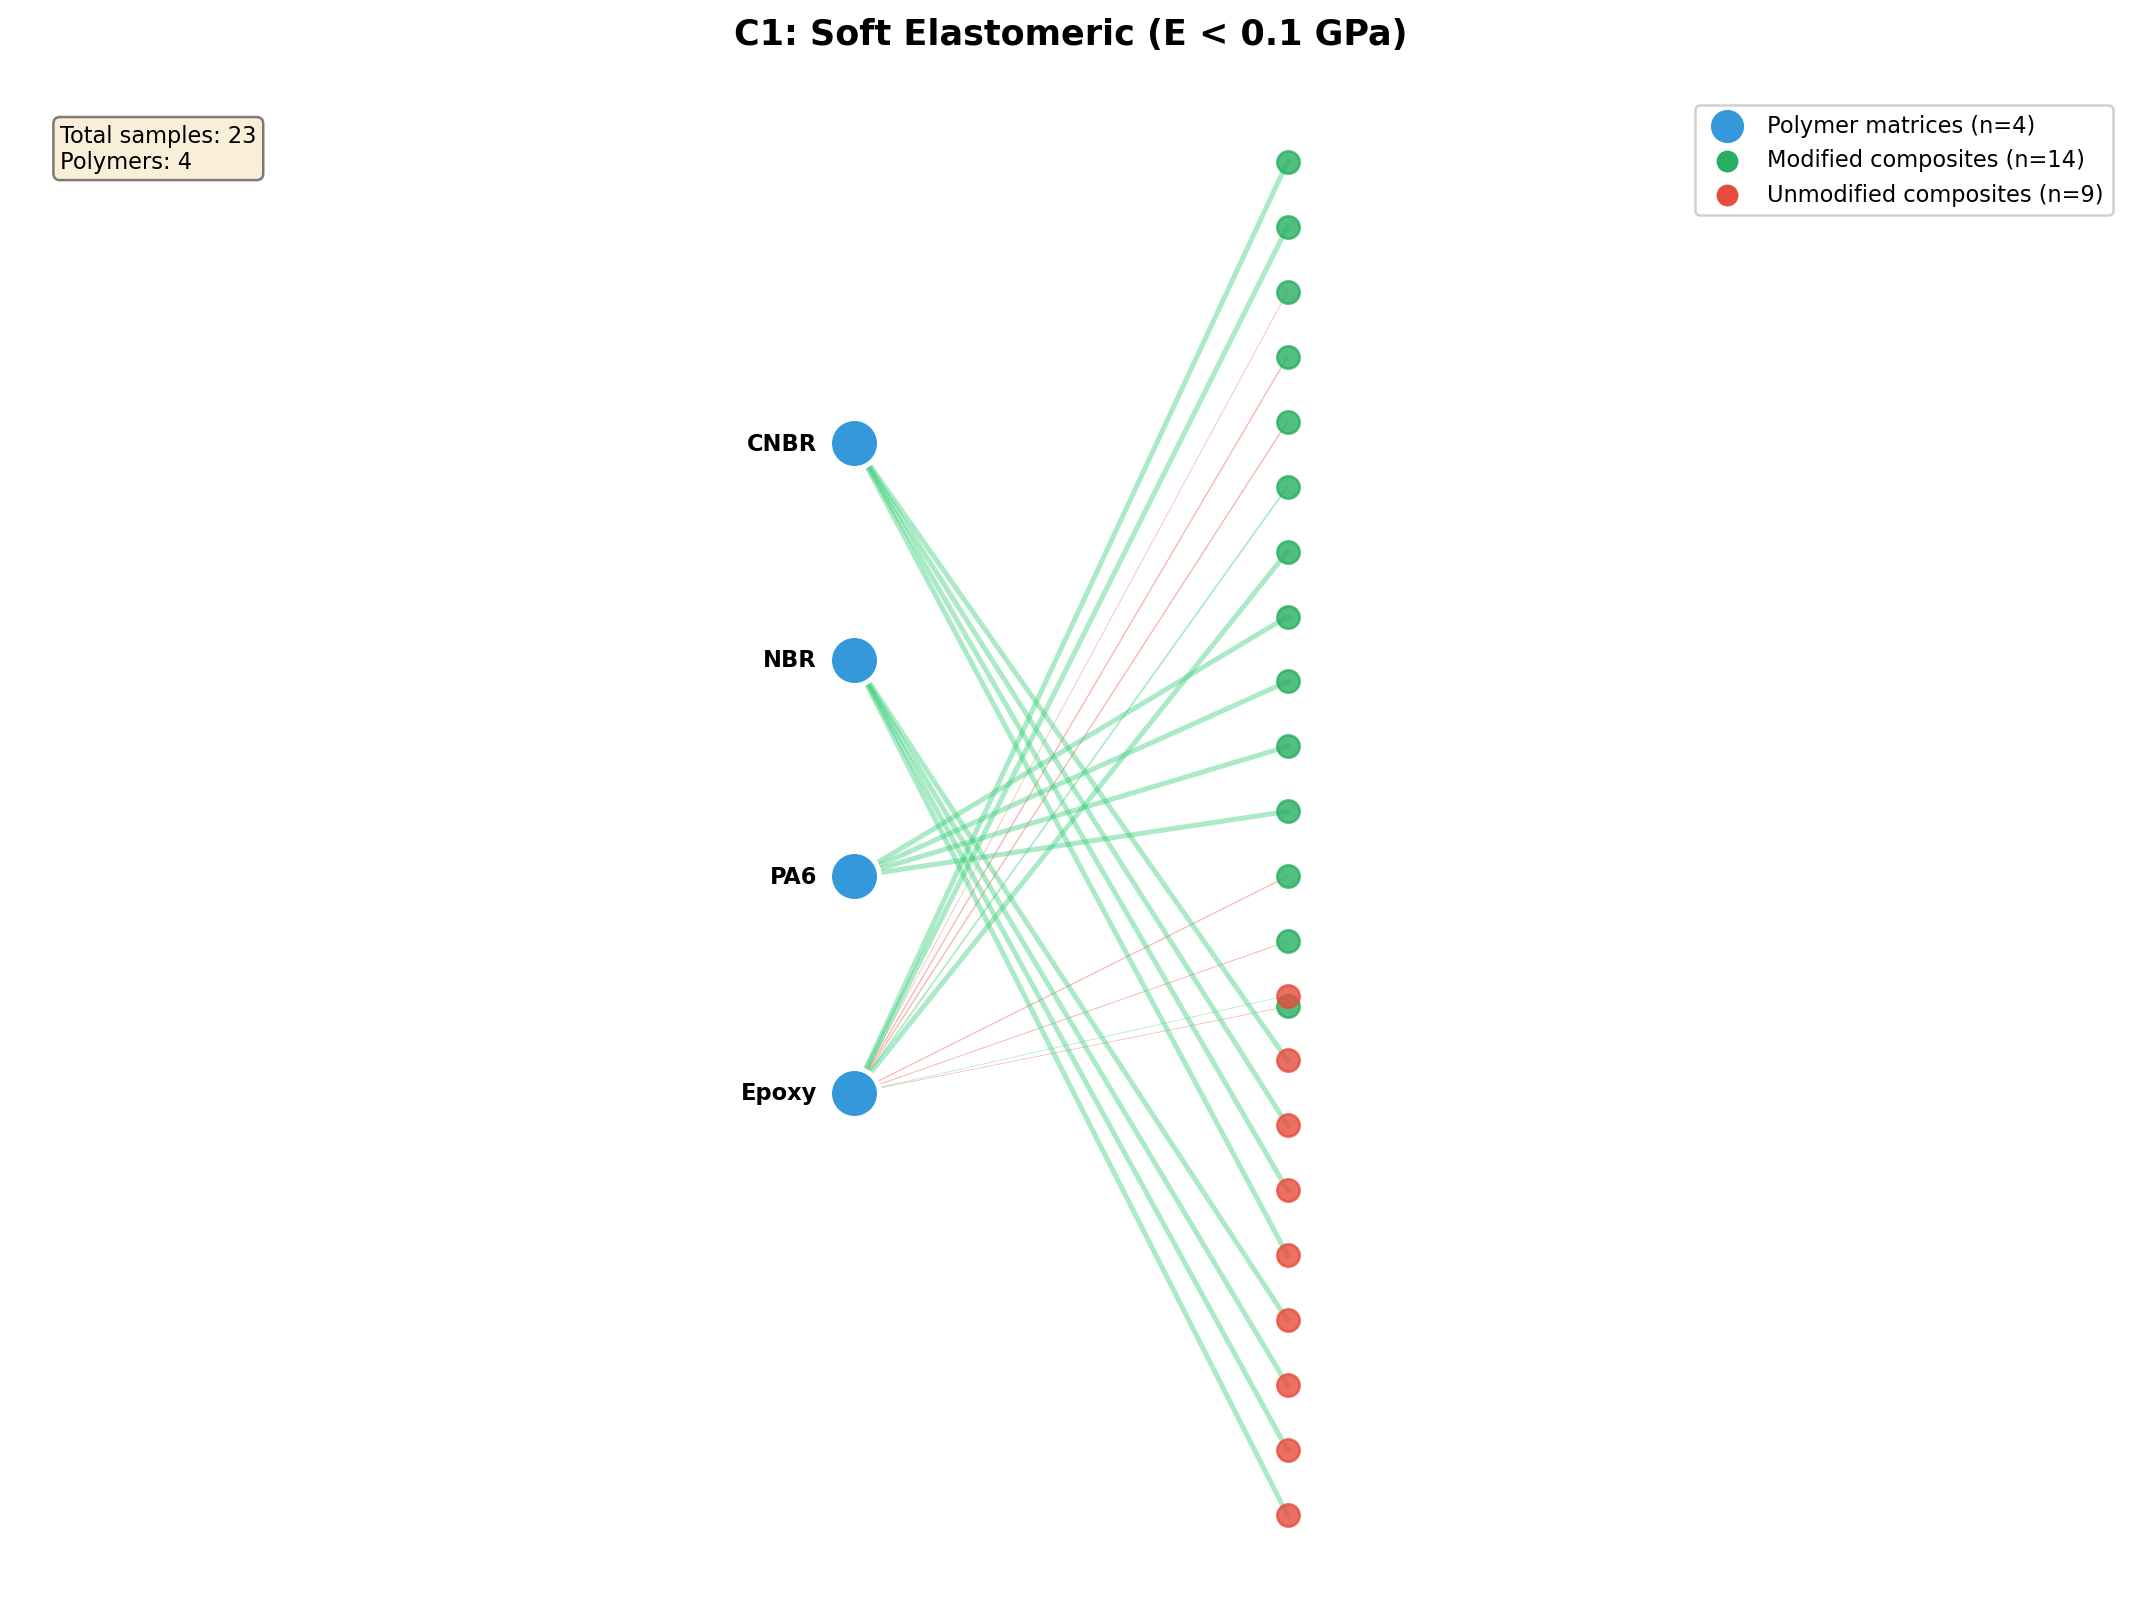
\includegraphics[width=0.23\textwidth]{cluster_C1_graph.png} &
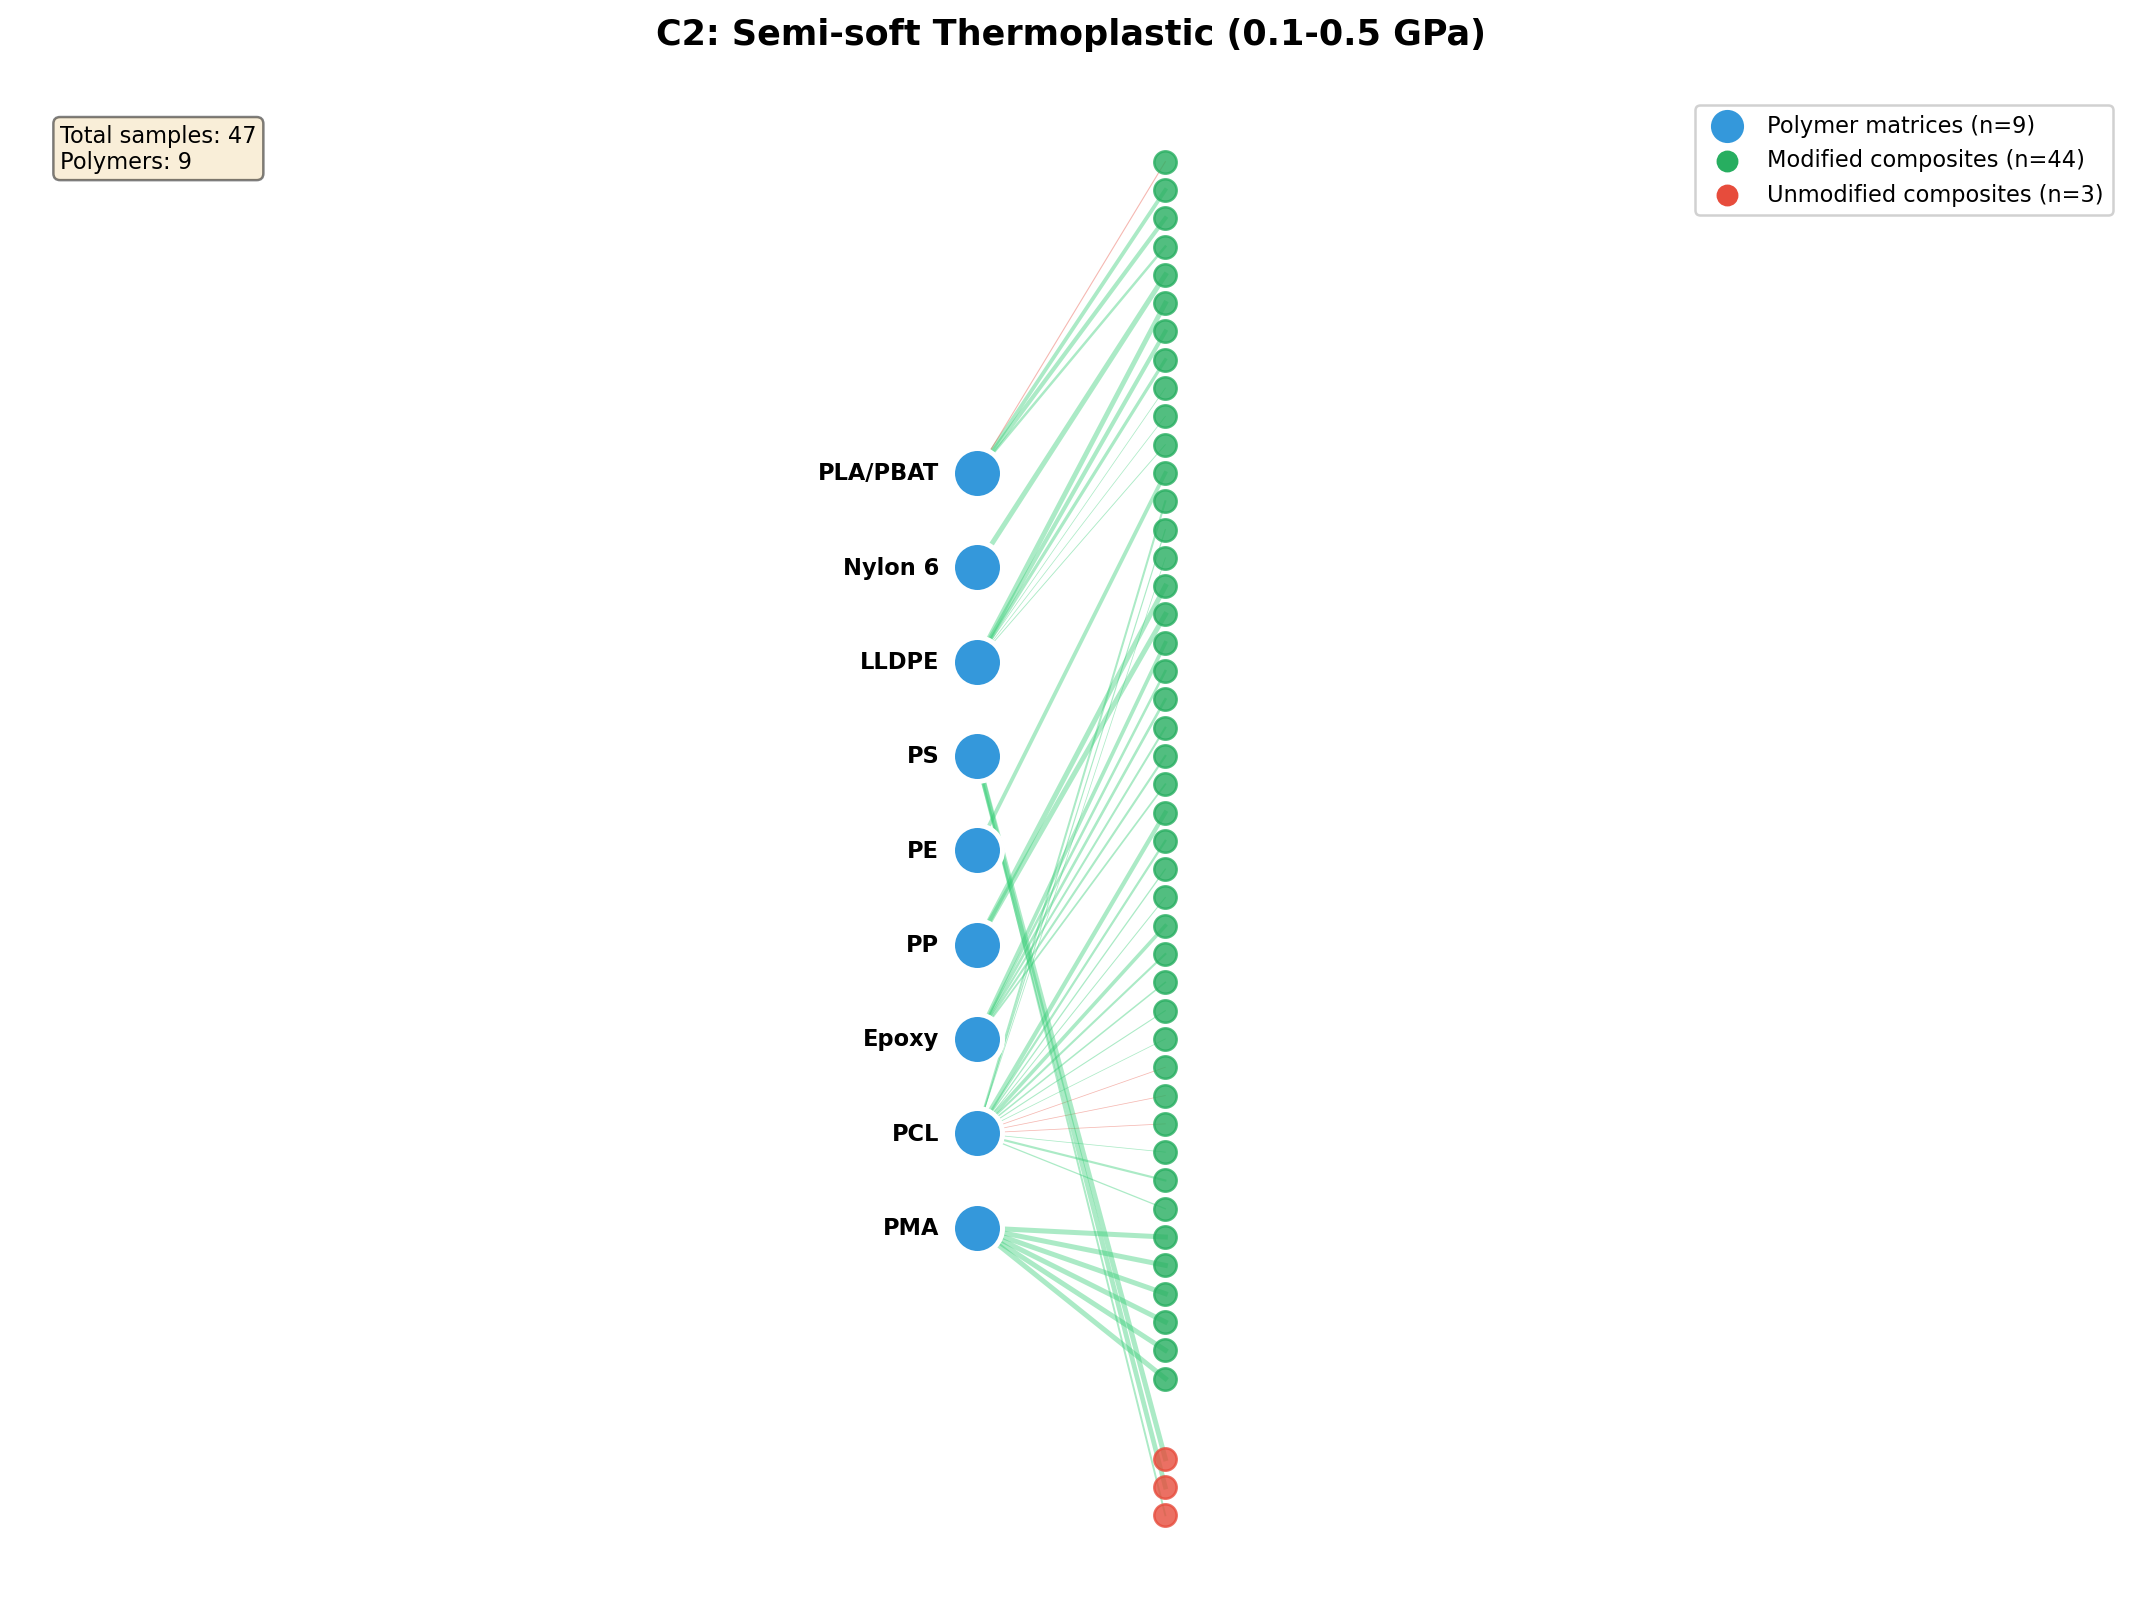
\includegraphics[width=0.23\textwidth]{cluster_C2_graph.png} \\
{\scriptsize (a) C1: Soft} & {\scriptsize (b) C2: Semi-soft} \\[2pt]
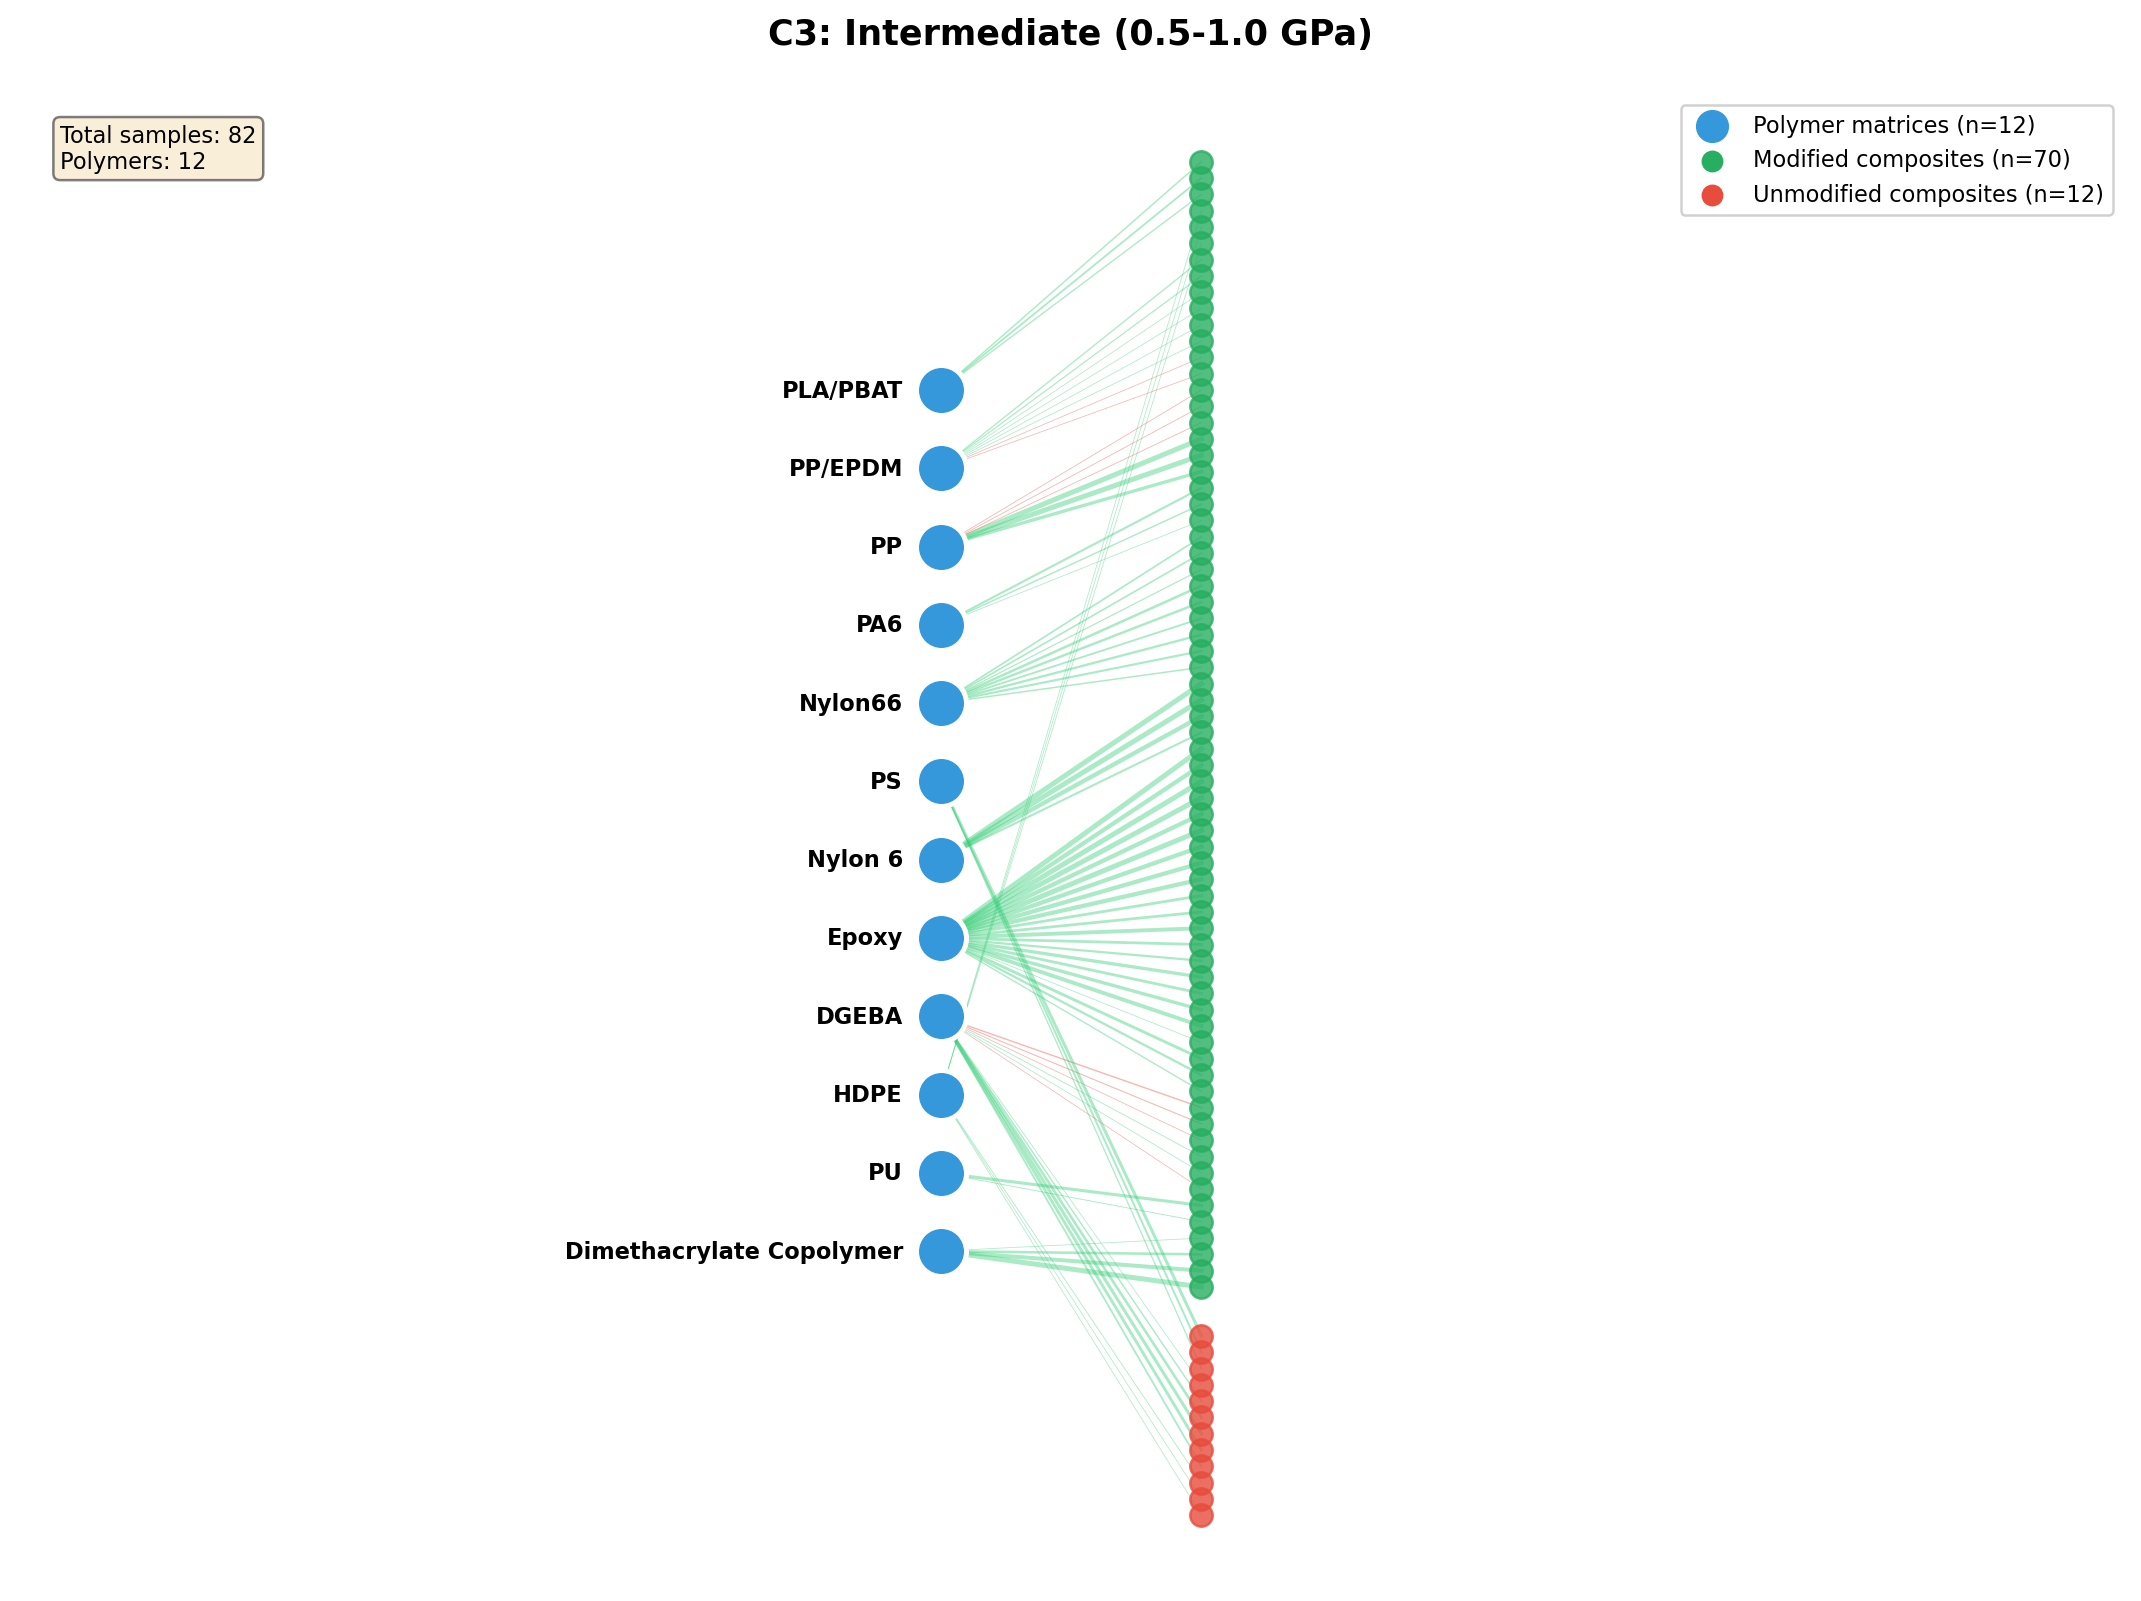
\includegraphics[width=0.23\textwidth]{cluster_C3_graph.png} &
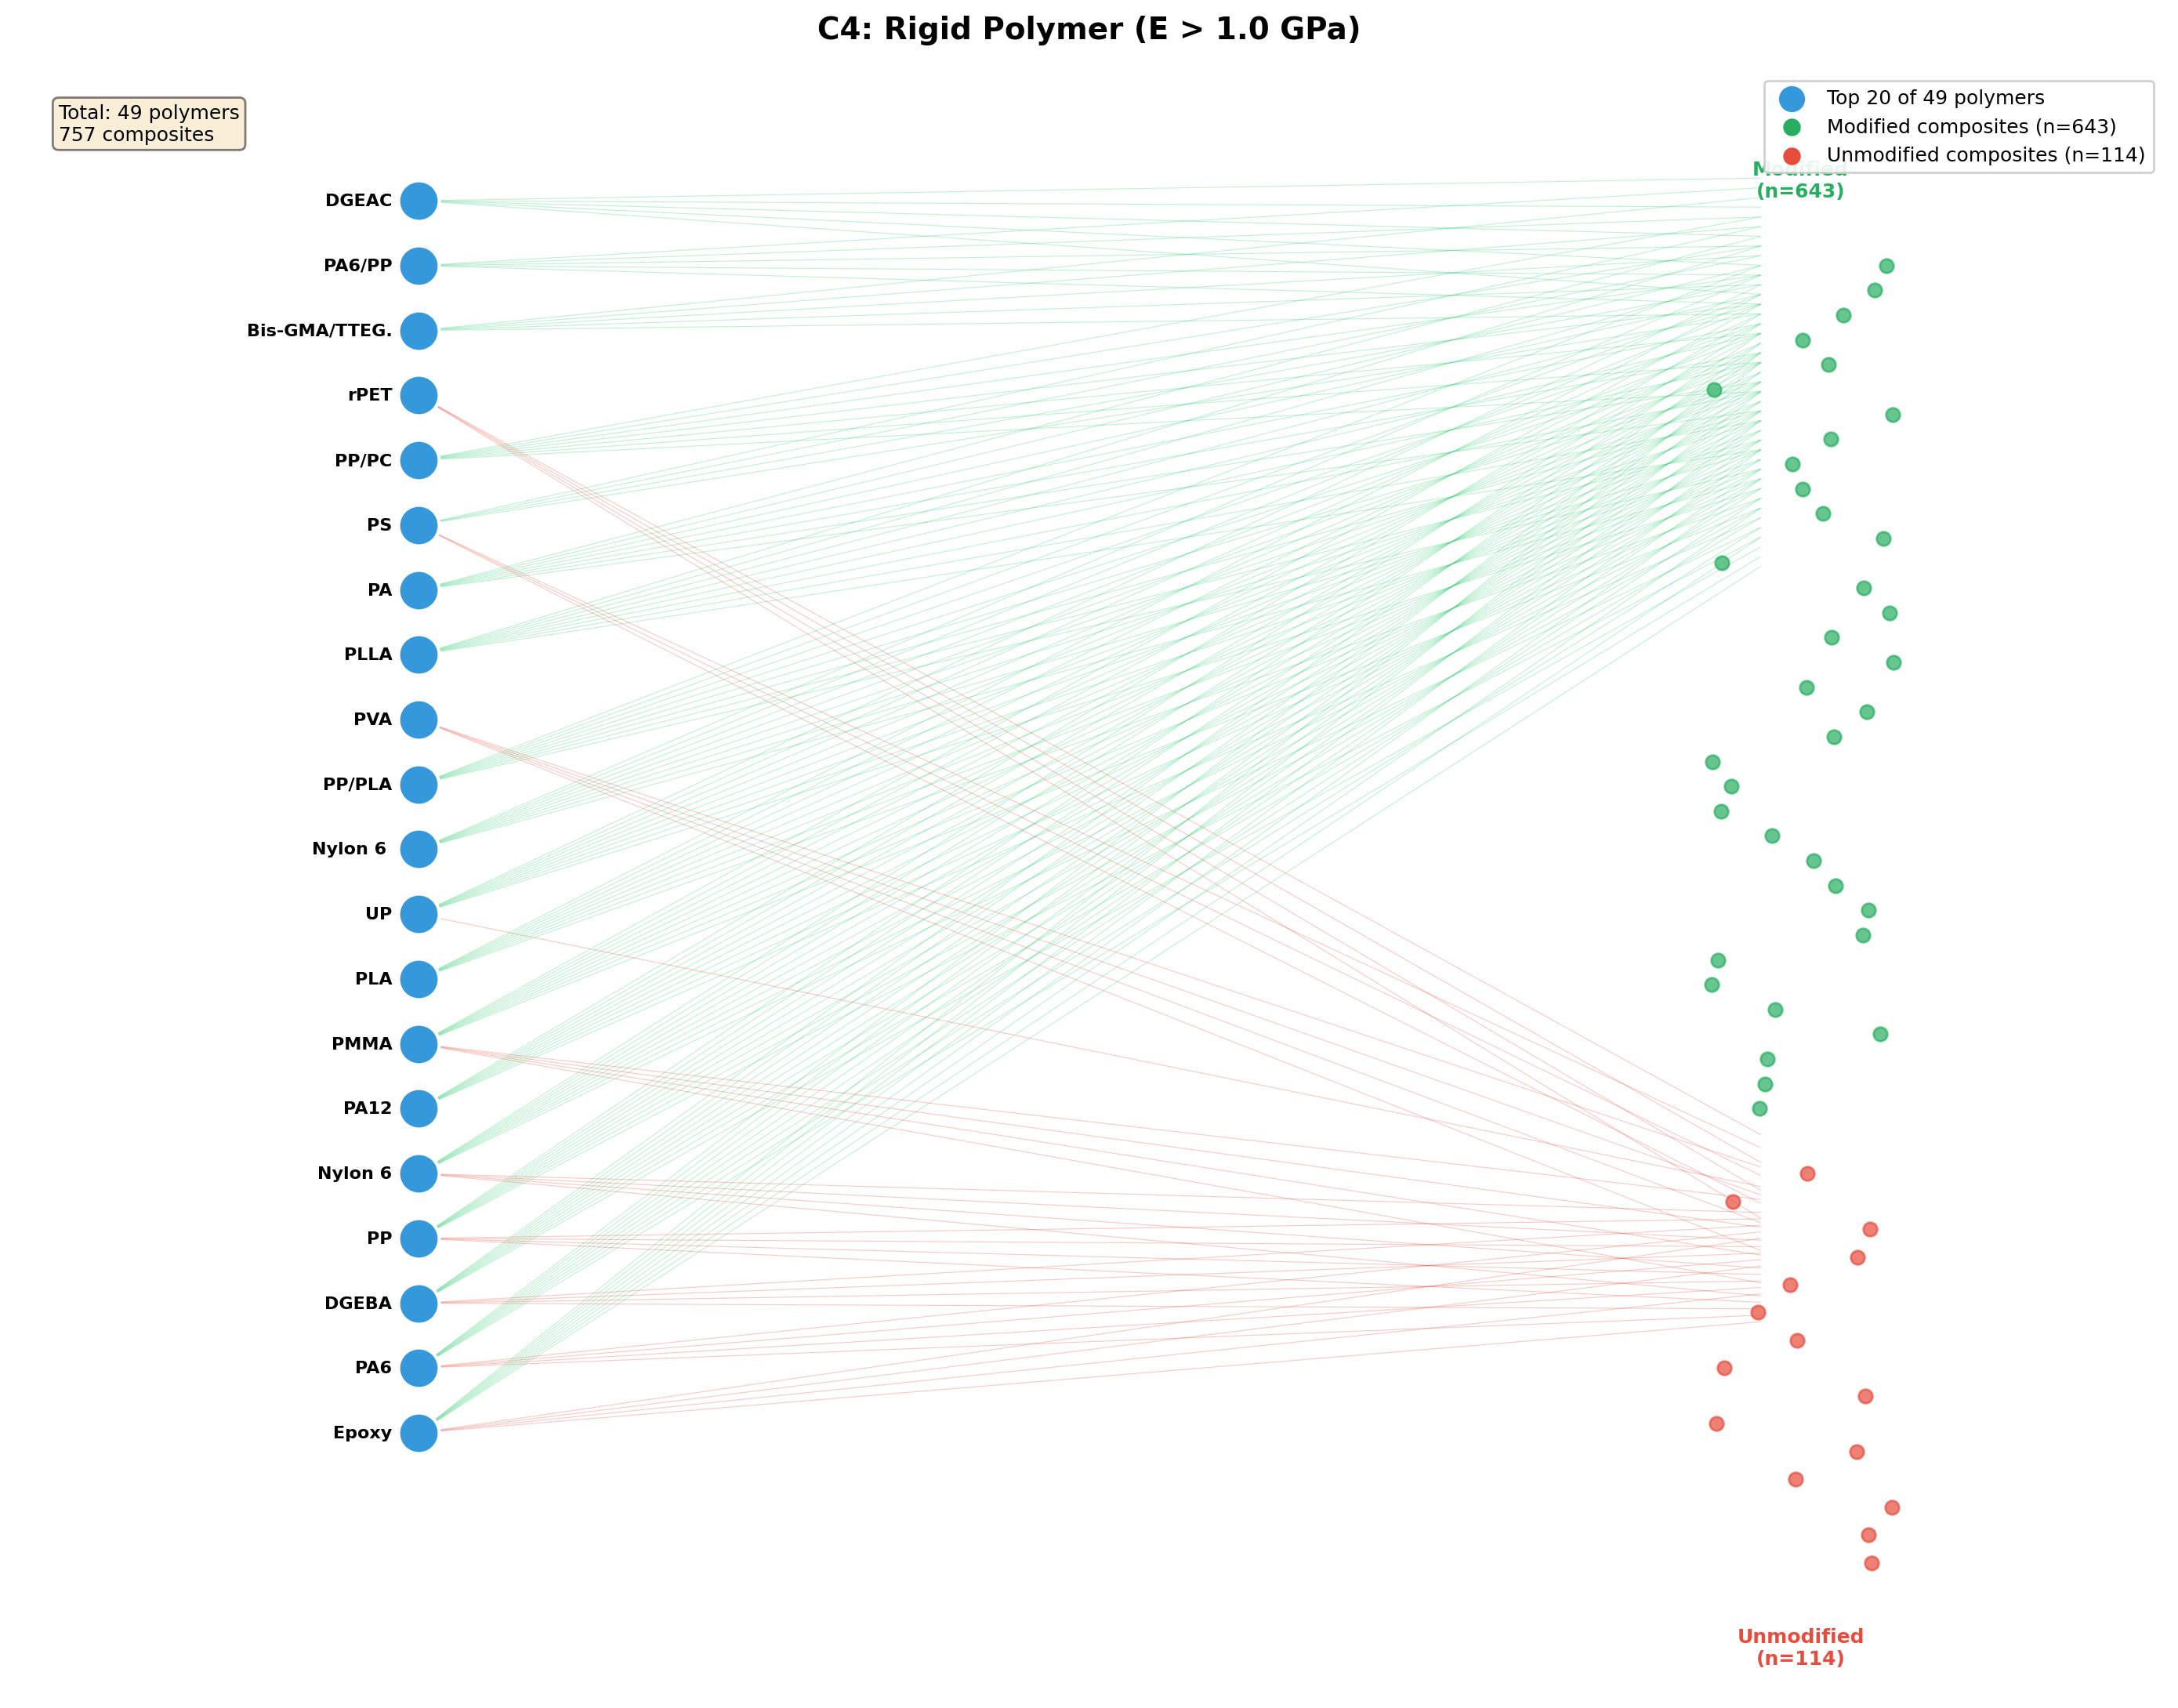
\includegraphics[width=0.23\textwidth]{cluster_C4_graph.png} \\
{\scriptsize (c) C3: Intermediate} & {\scriptsize (d) C4: Rigid} \\
\end{tabular}
\caption{Bipartite network graphs for each cluster. Blue nodes represent polymer matrices, green nodes indicate modified composites, red nodes denote unmodified samples.}
\label{fig:cluster_graphs}
\end{figure}

\subsection{Knowledge Hub Identification}

Centrality analysis identified distinct knowledge hubs within each cluster, as presented in Table~\ref{tab:centrality}. In Cluster C1, PA6 (polyamide 6) serves as the primary knowledge hub, with the highest weighted degree centrality (3822.86), indicating substantial property enhancements in soft matrix formulations \cite{64, 80, 107, 118}. Notably, while bulk PA6 typically demonstrates modulus values of 2-3 GPa, certain PA6 samples in the dataset represent plasticized or moisture-conditioned grades with significantly lower modulus values ($E_m \leq 0.1$ GPa) \cite{117, 129, 133, 141}. These low-modulus PA6 variants demonstrate considerable reinforcement potential when combined with clay nanofillers \cite{88, 124}.

\begin{table}[htbp]
\caption{Top Polymer Knowledge Hubs by Cluster}
\begin{center}
\begin{tabular}{@{}llccc@{}}
\toprule
Cluster & Polymer & $C_D$ & $C_{WD}$ & $C_B$ \\
\midrule
\multirow{2}{*}{C1} & PA6 & 0.154 & 3822.9 & 0.019 \\
 & CNBR & 0.154 & 2076.4 & 0.019 \\
\midrule
\multirow{2}{*}{C2} & PMA & 0.109 & 12318.2 & 0.010 \\
 & PCL & 0.327 & 527.8 & 0.103 \\
\midrule
\multirow{2}{*}{C3} & Epoxy & 0.237 & 1517.1 & 0.054 \\
 & Nylon 6 & 0.043 & 511.3 & 0.001 \\
\midrule
\multirow{2}{*}{C4} & Epoxy & 0.268 & 6386.1 & 0.072 \\
 & PA6 & 0.143 & 5285.0 & 0.020 \\
\bottomrule
\end{tabular}
\label{tab:centrality}
\end{center}
\end{table}

Cluster C2 identifies PMA as the dominant hub, exhibiting a weighted degree of 12318.18 \cite{1}, thereby indicating substantial property enhancements resulting from surface functionalization. In clusters C3 and C4, epoxy functions as the principal knowledge hub \cite{47, 49, 92}, achieving the highest degree centrality values (0.237 and 0.268), which reflects an extensive range of experimental research.

\subsection{Surface Modification Effectiveness}

A principal finding demonstrates that the effectiveness of surface modification strategies depends on material stiffness \cite{69, 107, 138}. Table~\ref{tab:modification} presents a comparison between modified and unmodified systems, including sample counts ($n_{mod}$ and $n_{unmod}$), included to contextualize the results. Surface modification yields the greatest benefit in Cluster C2 (semi-soft thermoplastics), where modified systems show a 222.6\% improvement over unmodified systems \cite{1, 90, 134}. This outcome, however, is derived from only three unmodified samples and should therefore be interpreted with caution. In contrast, the C4 cluster provides the most statistically robust comparison, with 643 modified and 114 unmodified samples \cite{80, 92, 127}.

\begin{table}[htbp]
\caption{Modified vs. Unmodified System Comparison}
\begin{center}
\footnotesize
\begin{tabular}{@{}lccccc@{}}
\toprule
Cluster & $n_m$ & $n_u$ & Mod. (\%) & Unmod. (\%) & Diff. (\%) \\
\midrule
C1 & 14 & 9 & 320.7 & 414.1 & -93.4 \\
C2 & 44 & 3 & 320.8 & 98.1 & +222.6 \\
C3 & 70 & 12 & 46.0 & 33.5 & +12.5 \\
C4 & 643 & 114 & 31.5 & 42.1 & -10.6 \\
\bottomrule
\end{tabular}
\label{tab:modification}
\end{center}
\end{table}

In C1 and C4, unmodified systems display greater average improvements, suggesting inherent matrix-clay compatibility \cite{19, 65, 132, 146}. The inverse relationship observed between matrix stiffness and the magnitude of improvement is consistent with composite mechanics \cite{10, 25, 112}. Softer matrices exhibit greater relative enhancement due to the larger modulus contrast with rigid clay platelets \cite{8, 11, 14, 22}.

\section{Limitations}

This study has several limitations. The bipartite graph structure yields disjoint star components, leading centrality metrics to primarily reflect sample counts and cumulative improvements rather than emergent network properties \cite{8, 11}. Confounding variables, including clay loading, morphology, and processing conditions, are not controlled \cite{10, 22, 92}. While meta-regression could improve causal interpretability, it falls outside the scope of this exploratory analysis \cite{68, 112, 127}. Sample sizes for unmodified composites are limited in certain clusters (C2: n=3), reducing statistical power \cite{91, 140}. The current edge weight formulation uses absolute values; future research should report positive and negative modulus changes separately \cite{14, 25}.

\section{Conclusion}

Graph-theoretic analysis provides a systematic method for evaluating polymer-clay nanocomposite research data compiled from 148 publications. The modulus-based clustering approach provides a physically meaningful framework for comparing materials with similar stiffness. Furthermore, bipartite graph construction effectively represents the relationships between polymer matrices and their composite formulations.

The principal findings are as follows: (1) An inverse relationship exists between matrix stiffness and the extent of property improvement, with soft systems (C1-C2) achieving average enhancements of 288-351\%, in contrast to 33-46\% for rigid polymers (C3-C4). (2) Key polymer systems serving as knowledge hubs with significant cumulative property enhancements include PA6 (C1), PMA (C2), and Epoxy (C3-C4). (3) The effectiveness of surface modification is influenced by matrix stiffness, as semi-soft thermoplastics (C2) exhibit the greatest benefit from modification (+222.6\%). This finding requires validation with larger unmodified sample sizes.

The methodology presented in this study provides a systematic framework for organizing heterogeneous literature data and identifying research patterns within the field of nanocomposites \cite{68, 91, 112, 127}. Subsequent research will expand this approach to include confounding variable analysis, normalized effect size metrics, and predictive modeling capabilities \cite{8, 22, 79, 116}.

\begin{thebibliography}{99}
\bibitem{1} J. E. Rauschendorfer et al., ``Tuning PMA properties via surface-functionalized MMT,'' \emph{Macromol. Mater. Eng.}, 2020.
\bibitem{2} J. J. Encalada-Alayola et al., ``Nanoclay effects on bis-GMA/TTEGDMA dental resins,'' \emph{Polymers}, vol. 12, 2020.
\bibitem{3} R. Arjmandi et al., ``Hybrid MMT/cellulose reinforced PLA nanocomposites,'' \emph{J. Mater. Sci.}, vol. 50, pp. 3118--3130, 2015.
\bibitem{4} L. R. de Menezes and E. O. da Silva, ``MMT clays for dental adhesives,'' \emph{Mater. Res.}, vol. 19, pp. 236--242, 2016.
\bibitem{5} V. S. Abhisha et al., ``HNT and bentonite effects on natural rubber,'' \emph{J. Elastomers Plast.}, vol. 52, pp. 432--452, 2020.
\bibitem{6} A. Kassa et al., ``Clay effects on PCL bionanocomposites,'' \emph{Polym. Polym. Compos.}, vol. 28, pp. 338--347, 2020.
\bibitem{7} A. C. Kandemir et al., ``Polymer/clay nanocomposite coatings,'' \emph{Polym. Compos.}, 2023.
\bibitem{8} Y. Zare and K. Y. Rhee, ``Young's modulus simulation for clay nanocomposites,'' \emph{J. Mater. Res. Technol.}, vol. 9, pp. 12473--12483, 2020.
\bibitem{9} Y. Zare and K. Y. Rhee, ``Polymer HNT nanocomposite modulus model,'' \emph{Sci. Rep.}, vol. 12, 2022.
\bibitem{10} Y. Q. Rao and J. M. Pochan, ``Mechanics of polymer-clay nanocomposites,'' \emph{Macromolecules}, vol. 40, pp. 290--296, 2007.
\bibitem{11} M. Heydari-Meybodi et al., ``3D multiscale modeling of polymer/nanoclay,'' \emph{Compos. Interfaces}, vol. 23, pp. 641--661, 2016.
\bibitem{12} Y. Zare and K. Y. Rhee, ``Hashin-Shtrikman model for clay/PP nanocomposite,'' \emph{Appl. Clay Sci.}, vol. 137, pp. 176--182, 2017.
\bibitem{13} Y. Zare, ``Percolation and interphase in polymer/clay nanocomposites,'' \emph{J. Colloid Interface Sci.}, vol. 486, pp. 249--254, 2017.
\bibitem{14} Y. Zare et al., ``Stress transfer efficiency in clay/polymer nanocomposites,'' \emph{Appl. Clay Sci.}, vol. 143, pp. 265--272, 2017.
\bibitem{15} B. Akbari and R. Bagheri, ``Deformation mechanism of epoxy/clay nanocomposite,'' \emph{Eur. Polym. J.}, vol. 43, pp. 782--788, 2007.
\bibitem{16} L. N. Carli et al., ``PHBV nanocomposites with MMT and halloysite,'' \emph{Compos. Part A}, vol. 42, pp. 1601--1608, 2011.
\bibitem{17} M. Heydari-Meybodi et al., ``Elastic modulus prediction with interfacial debonding,'' \emph{Compos. Sci. Technol.}, vol. 117, pp. 379--385, 2015.
\bibitem{18} R. M. Moghadam et al., ``Clay-epoxy nanocomposite tensile behavior,'' \emph{Compos. Part B}, vol. 89, pp. 303--315, 2016.
\bibitem{19} Y. Zare and K. Y. Rhee, ``Interfacial shear modulus effects,'' \emph{Constr. Build. Mater.}, vol. 247, 2020.
\bibitem{20} C. J. G. Plummer et al., ``PU nanocomposites with hyperbranched polymers,'' \emph{Polymer}, pp. 6543--6553, 2005.
\bibitem{21} M. Morits et al., ``Nacre-mimetic clay/polymer nanocomposites,'' \emph{Adv. Funct. Mater.}, vol. 27, 2017.
\bibitem{22} F. Za\"{i}ri et al., ``Multiscale modeling of polymer/clay nanocomposites,'' \emph{Acta Mater.}, vol. 59, pp. 3851--3863, 2011.
\bibitem{23} M. Silani et al., ``Clay/epoxy nanocomposites investigation,'' \emph{Compos. Struct.}, vol. 94, pp. 3142--3148, 2012.
\bibitem{24} A. Yasmin et al., ``Clay/epoxy nanocomposite behavior,'' \emph{Compos. Sci. Technol.}, vol. 66, pp. 2415--2422, 2006.
\bibitem{25} M. L. Chan et al., ``Reinforcement mechanism in nanoclay/polymer,'' \emph{Compos. Part B}, vol. 42, pp. 1708--1712, 2011.
\bibitem{26} H. Alamri and I. M. Low, ``Water absorption effects on epoxy nanocomposites,'' \emph{Mater. Des.}, vol. 42, pp. 214--222, 2012.
\bibitem{27} S. Zainuddin et al., ``Nanoclay-epoxy flexural properties,'' \emph{Mater. Sci. Eng. A}, vol. 527, pp. 7920--7926, 2010.
\bibitem{28} S. B. Basturk and S. C. Erbas, ``Nanoclay/epoxy thermo-mechanical properties,'' \emph{Mater. Res. Express}, vol. 5, 2018.
\bibitem{29} T. K. B. Sharmila et al., ``Cloisite epoxy nanocomposites,'' \emph{Appl. Clay Sci.}, vol. 102, pp. 220--230, 2014.
\bibitem{30} Y. Ali et al., ``Degassing and nanoclay effects on epoxy,'' \emph{Defect Diffus. Forum}, pp. 237--243, 2015.
\bibitem{31} M. Al-Qadhi et al., ``Water and crude oil effects on epoxy-clay,'' \emph{Polym. Compos.}, vol. 35, pp. 318--326, 2014.
\bibitem{32} M. Esteves et al., ``Tribological behavior of epoxy/nanoclay,'' \emph{Tribol. Lett.}, vol. 52, pp. 1--10, 2013.
\bibitem{33} A. Jumahat et al., ``Nanoclay modified aerospace epoxy,'' \emph{Plast. Rubber Compos.}, vol. 41, pp. 225--232, 2012.
\bibitem{34} A. Jumahat et al., ``Nanoclay/epoxy compressive properties,'' \emph{Procedia Eng.}, pp. 1607--1613, 2012.
\bibitem{35} A. Jumahat et al., ``Nanoclay-modified epoxy flexural response,'' \emph{Mater. Res. Innov.}, vol. 18, 2014.
\bibitem{36} M. A. Kumar et al., ``Epoxy/clay with glass fiber,'' \emph{Int. J. Polym. Mater.}, vol. 59, pp. 854--862, 2010.
\bibitem{37} C. K. Lam and K. T. Lau, ``Nanoclay clusters in epoxy,'' \emph{J. Thermoplast. Compos. Mater.}, vol. 22, pp. 213--225, 2009.
\bibitem{38} X. Li et al., ``Exfoliated epoxy/clay nanocomposites,'' \emph{Polym. Bull.}, vol. 67, pp. 719--727, 2011.
\bibitem{39} M. Al-Qadhi et al., ``Epoxy-clay water uptake,'' \emph{J. Mater. Sci.}, vol. 48, pp. 3798--3804, 2013.
\bibitem{40} R. Aradhya and N. M. Renukappa, ``Epoxy nanocomposites for HV applications,'' \emph{IntechOpen}, 2020.
\bibitem{41} T. P. Mohan et al., ``Epoxy-clay thermal and mechanical properties,'' \emph{J. Mater. Sci.}, vol. 41, pp. 5915--5925, 2006.
\bibitem{42} A. Okada and A. Usuki, ``Twenty years of polymer-clay nanocomposites,'' \emph{Macromol. Mater. Eng.}, vol. 291, pp. 1449--1476, 2006.
\bibitem{43} D. Ratna et al., ``Clay-reinforced epoxy nanocomposites,'' \emph{Polym. Int.}, vol. 52, pp. 1403--1407, 2003.
\bibitem{44} Rashmi et al., ``OMMT filled epoxy wear behaviour,'' \emph{Mater. Des.}, vol. 32, pp. 4528--4536, 2011.
\bibitem{45} N. Rull et al., ``Nanoclays on glass fiber/UP composites,'' \emph{J. Compos. Mater.}, vol. 49, pp. 1629--1637, 2015.
\bibitem{46} R. Jeyakumar et al., ``Glass fiber epoxy nanoclay composites,'' \emph{Int. J. Adv. Manuf. Technol.}, vol. 93, pp. 527--535, 2017.
\bibitem{47} M. Shettar et al., ``Nanoclay-epoxy mechanical properties,'' \emph{J. Mater. Res. Technol.}, vol. 9, pp. 9108--9116, 2020.
\bibitem{48} M. Shettar et al., ``Hygrothermal aging of GF-epoxy-nanoclay,'' \emph{Mater. Res. Express}, vol. 7, 2020.
\bibitem{49} A. Tcherbi-Narteh et al., ``MMT nanoclay effects on DGEBA epoxy,'' \emph{J. Nanomater.}, 2016.
\bibitem{50} M. Shettar et al., ``Water sorption effects on epoxy-nanoclay,'' \emph{Int. J. Automot. Mech. Eng.}, vol. 19, pp. 9478--9486, 2022.
\bibitem{51} C. Wolf et al., ``Filler shape effects on barrier properties,'' \emph{J. Membr. Sci.}, vol. 556, pp. 393--418, 2018.
\bibitem{52} J. Zhang et al., ``Nanoparticles and CTBN in epoxy toughening,'' \emph{Compos. Part A}, vol. 80, pp. 82--94, 2016.
\bibitem{53} S. Firdosh et al., ``Nano-gelcoat water absorption,'' \emph{Prog. Org. Coat.}, vol. 114, pp. 173--187, 2018.
\bibitem{54} M. H. Mat Yazik et al., ``Nanoclay effects on epoxy shape memory,'' \emph{Polym. Bull.}, vol. 77, pp. 5913--5931, 2020.
\bibitem{55} S. Fakhreddini-Najafabadi et al., ``Synthesis effects on nanoclay/epoxy,'' \emph{J. Mater. Res. Technol.}, vol. 15, pp. 5375--5395, 2021.
\bibitem{56} K. M\"{u}ller et al., ``Polymer nanocomposites review,'' \emph{Nanomaterials}, vol. 7, 2017.
\bibitem{57} A. D. de Oliveira and C. A. G. Beatrice, ``Polymer nanocomposites with nanofillers,'' \emph{IntechOpen}, 2019.
\bibitem{58} A. Cerit et al., ``Epoxide modification effects on epoxy,'' \emph{Int. J. Polym. Sci.}, 2016.
\bibitem{59} N. Domun et al., ``Epoxy fracture toughness with nanomaterials,'' \emph{Nanoscale}, vol. 7, pp. 10294--10329, 2015.
\bibitem{60} X. Jia et al., ``Moisture-resistant epoxy with activated MMT,'' \emph{RSC Adv.}, vol. 5, pp. 44853--44864, 2015.
\bibitem{61} S. Kowshik et al., ``Nanoclay effects on GF-epoxy,'' \emph{Cogent Eng.}, vol. 9, 2022.
\bibitem{62} Kusmono and Z. A. M. Ishak, ``Clay on UP/glass fiber composites,'' \emph{Int. J. Polym. Sci.}, 2013.
\bibitem{63} T. A. Nguyen et al., ``Epoxy with nanoclay I.30E,'' \emph{J. Chem.}, 2020.
\bibitem{64} A. M. Abdel-Gawad et al., ``Nylon 6-MMT nanocomposites,'' \emph{Polymers}, vol. 14, 2022.
\bibitem{65} N. Merah and O. Mohamed, ``Nanoclay effects on unsaturated polyester,'' \emph{J. Nanomater.}, 2019.
\bibitem{66} G. \"{O}r\c{c}en and D. Bayram, ``Nanoclay on GF-epoxy composites,'' \emph{J. Mater. Sci.}, vol. 59, pp. 3467--3487, 2024.
\bibitem{67} P. Saikia, ``Clay nanostructures for biomedical applications,'' \emph{Elsevier}, 2019.
\bibitem{68} S. S. Ray, ``Clay-containing polymer nanocomposites trends,'' \emph{Macromol. Chem. Phys.}, vol. 215, pp. 1162--1179, 2014.
\bibitem{69} S. S. Chee and M. Jawaid, ``Bi-functionalized MMT on epoxy nanocomposites,'' \emph{Polymers}, vol. 11, 2019.
\bibitem{70} P. N. Harshita et al., ``Nanoclay/epoxy at elevated temperatures,'' \emph{Trans. Indian Inst. Met.}, vol. 71, pp. 2015--2024, 2018.
\bibitem{71} I. Ozsoy et al., ``Micro/nano-filler effects on epoxy,'' \emph{Stroj. Vestn.}, vol. 61, pp. 601--609, 2015.
\bibitem{72} Z. S. Kiran et al., ``Cloisite 15A reinforced epoxy-glass,'' \emph{Iran. Polym. J.}, vol. 30, pp. 831--841, 2021.
\bibitem{73} J. Zicans et al., ``Thermoplastic polymer nanocomposite modeling,'' \emph{ZAMM}, vol. 95, pp. 1198--1110, 2015.
\bibitem{74} R. M. Meri et al., ``rPET/MMT composites,'' \emph{Compos. Struct.}, vol. 111, pp. 453--458, 2014.
\bibitem{75} H. W. Wang et al., ``Particle-reinforced polymer FEM,'' \emph{Adv. Mater. Res.}, pp. 2177--2180, 2011.
\bibitem{76} R. D. Maksimov and E. Plume, ``PU/MMT nanocomposite elastic properties,'' 2012.
\bibitem{77} H. Ebadi-Dehaghani et al., ``PP/PLA/clay nanocomposite properties,'' \emph{Compos. Part B}, vol. 69, pp. 133--144, 2015.
\bibitem{78} R. Mohsenzadeh, ``PA6/zeolite nanocomposite properties,'' \emph{Proc. IMechE Part C}, vol. 235, pp. 7233--7240, 2021.
\bibitem{79} B. Zazoum et al., ``DNN modeling of clay nanocomposites,'' \emph{Materials}, vol. 13, 2020.
\bibitem{80} A. N. Wilkinson et al., ``PA6-MMT nanocomposite tensile properties,'' \emph{Compos. Sci. Technol.}, vol. 67, pp. 3360--3368, 2007.
\bibitem{81} M. Jamsheed et al., ``MMT nanoclay on CF/epoxy laminates,'' \emph{Polym. Compos.}, 2025.
\bibitem{82} G. Ravichandran et al., ``Epoxy/HNT nanocomposites,'' \emph{SN Appl. Sci.}, vol. 1, 2019.
\bibitem{83} S. Ghafarloo and M. Kokabi, ``Epoxy clay nanocomposite properties,'' \emph{Adv. Mater. Res.}, pp. 145--148, 2010.
\bibitem{84} A. E. Jahromi et al., ``PA/clay nanocomposites with NBR,'' \emph{Compos. Part B}, vol. 90, pp. 478--484, 2016.
\bibitem{85} P. M. Gyoo et al., ``PA66/clay with epoxy-modified organoclay,'' \emph{J. Appl. Polym. Sci.}, vol. 101, pp. 1711--1722, 2006.
\bibitem{86} R. Aradhya and N. M. Renukappa, ``Epoxy nanocomposites tribology,'' \emph{IntechOpen}, 2020.
\bibitem{87} J. Stoj\v{s}i\'{c} et al., ``PA12/clay nanocomposite structure,'' \emph{Polym. Compos.}, vol. 37, pp. 684--691, 2016.
\bibitem{88} M. H. Gabr and K. Uzawa, ``PA/nanoclay nanocomposite properties,'' \emph{J. Thermoplast. Compos. Mater.}, vol. 31, pp. 447--464, 2018.
\bibitem{89} R. C. Voicu et al., ``Nano-clay biopolymeric composite prediction,'' \emph{Nanomaterials}, vol. 14, 2024.
\bibitem{90} L. Su et al., ``Functionalized MMT/epoxy nanocomposites,'' \emph{RSC Adv.}, vol. 14, pp. 31251--31258, 2024.
\bibitem{91} E. Manias et al., ``PP/MMT nanocomposites review,'' \emph{Chem. Mater.}, vol. 13, pp. 3516--3523, 2001.
\bibitem{92} A. A. Azeez et al., ``Epoxy clay nanocomposites review,'' \emph{Compos. Part B}, vol. 45, pp. 308--320, 2013.
\bibitem{93} A. Nordin et al., ``Nanoclay loading effects on nanocomposites,'' 2015.
\bibitem{94} E. Esmizadeh et al., ``PP/PC/clay nanocomposites,'' \emph{Sci. Eng. Compos. Mater.}, vol. 25, pp. 31--39, 2018.
\bibitem{95} M. R. Nakhaei et al., ``PP/EPDM/clay optimization,'' \emph{Polym. Compos.}, vol. 38, pp. E421--E432, 2017.
\bibitem{96} J. Huang et al., ``PA6 nanoparticle RVE modeling,'' \emph{J. Mater. Sci. Chem. Eng.}, vol. 3, pp. 95--102, 2015.
\bibitem{97} J.-I. Weon, ``PA6/clay micromechanical modeling,'' 2009.
\bibitem{98} E. Amendola, ``Silylated MMT epoxy nanocomposites,'' \emph{Open Macromol. J.}, vol. 6, pp. 33--36, 2012.
\bibitem{99} M. Moghri et al., ``PA6/clay parameters via GA and RSM,'' \emph{Int. Nano Lett.}, vol. 5, pp. 133--140, 2015.
\bibitem{100} S. Bayar et al., ``Temperature effects on nanoclay/polymer,'' 2010.
\bibitem{101} X. Liu et al., ``PA6-clay/PP-g-MA alloys,'' \emph{Polymer}, 2001.
\bibitem{102} M. Quaresimin et al., ``Clay-modified epoxy fracture,'' \emph{Eng. Fract. Mech.}, vol. 81, pp. 80--93, 2012.
\bibitem{103} M. A. P\'{e}rez et al., ``PP/clay nanocomposites synthesis,'' 2010.
\bibitem{104} I. M. Daniel et al., ``Epoxy/clay nanocomposites processing,'' 2006.
\bibitem{105} H. U. Zaman et al., ``PP/clay with compatibilizers,'' \emph{J. Thermoplast. Compos. Mater.}, vol. 27, pp. 338--349, 2014.
\bibitem{106} J. Stoj\v{s}i\'{c} et al., ``PA12/clay flexural properties,'' \emph{Polymers}, vol. 14, 2022.
\bibitem{107} E. Naveau et al., ``Clay modification on PA6 nanocomposites,'' \emph{Eur. Polym. J.}, vol. 47, pp. 5--15, 2011.
\bibitem{108} L. B. Manfredi et al., ``MMT on GF/epoxy properties,'' \emph{Compos. Part A}, vol. 39, pp. 1726--1731, 2008.
\bibitem{109} M. Dua and P. Mertiny, ``Elastomer clay nanocomposite models,'' 2021.
\bibitem{110} C. Jo and H. E. Naguib, ``Polymer/clay nanocomposite foams,'' \emph{J. Phys. Conf. Ser.}, vol. 61, pp. 861--868, 2007.
\bibitem{111} ``PA6/clay nanocomposites critical review,'' 2010.
\bibitem{112} S. S. Ray and M. Okamoto, ``Polymer/layered silicate nanocomposites review,'' \emph{Prog. Polym. Sci.}, vol. 28, pp. 1539--1641, 2003.
\bibitem{113} ``Nanoclay on thin polymer composite perforation,'' 2012.
\bibitem{114} M. Chinnapandi et al., ``GF reinforced polymer-clay properties,'' \emph{J. Phys. Conf. Ser.}, 2024.
\bibitem{115} A. P. Sharma et al., ``GFRP-polymer sandwich with MMT,'' \emph{J. Phys. Conf. Ser.}, 2024.
\bibitem{116} M. Akbarzadeh et al., ``ML optimization of PLA/PBAT/clay,'' \emph{Polym. Eng. Sci.}, 2024.
\bibitem{117} L. Shen et al., ``Nylon-6 nanocomposite nanoindentation,'' \emph{Polymer}, vol. 46, pp. 11969--11977, 2005.
\bibitem{118} J. W. Cho and D. R. Paul, ``Nylon 6 nanocomposites by melt compounding,'' \emph{Polymer}, 2001.
\bibitem{119} A. Ranade et al., ``Nylon-6 and MLS nanocomposites,'' \emph{J. Plast. Film Sheeting}, vol. 19, pp. 271--285, 2003.
\bibitem{120} T. V. Gonz\'{a}lez et al., ``Nylon 6/organoclay by extrusion,'' \emph{J. Appl. Polym. Sci.}, vol. 108, pp. 2923--2933, 2008.
\bibitem{121} D. Shah et al., ``PA6 nanocomposite via solid-state shear pulverization,'' \emph{Polymer}, vol. 45, pp. 2991--3000, 2004.
\bibitem{122} H. M. Koo et al., ``HDPE/MMT nanocomposites morphology,'' \emph{Fibers Polym.}, vol. 8, pp. 68--72, 2007.
\bibitem{123} V. A. F. Costa, ``GFRP composites: production, modeling, application,'' \emph{Materials}, 2022.
\bibitem{124} T. D. Fornes and D. R. Paul, ``Modeling nylon 6/clay nanocomposite properties,'' \emph{Polymer}, vol. 44, pp. 4993--5013, 2003.
\bibitem{125} D. Jia et al., ``Polyolefin clay nanocomposites synthesis,'' \emph{Polym. Compos.}, vol. 25, pp. 312--318, 2004.
\bibitem{126} S.-S. Ray and M. Bousmina, ``PBSA/MMT nanocomposites,'' \emph{Macromol. Chem. Phys.}, vol. 206, pp. 1674--1684, 2005.
\bibitem{127} D. R. Paul and L. M. Robeson, ``Polymer nanotechnology: nanocomposites,'' \emph{Polymer}, vol. 49, pp. 3187--3204, 2008.
\bibitem{128} H. E. Miltner et al., ``Isotactic PP crystallization with MMT,'' \emph{Polymer}, vol. 47, pp. 826--835, 2006.
\bibitem{129} M. Lai et al., ``PA6 crystallization with clays,'' \emph{J. Appl. Polym. Sci.}, vol. 105, pp. 2456--2462, 2007.
\bibitem{130} T. S. Ellis and J. S. D'Angelo, ``Epoxy-silicate nanocomposites,'' \emph{J. Appl. Polym. Sci.}, vol. 90, pp. 1639--1647, 2003.
\bibitem{131} S. C. Lee and K. Y. Rhee, ``HDPE/MMT nanocomposite study,'' \emph{Polym. Adv. Technol.}, vol. 20, pp. 1040--1045, 2009.
\bibitem{132} M. A. Osman et al., ``PE/clay gas permeation,'' \emph{Macromolecules}, vol. 37, pp. 9489--9496, 2004.
\bibitem{133} J. I. Weon, ``PA6/clay nanocomposite creep behavior,'' \emph{Polymer}, vol. 49, pp. 2463--2467, 2008.
\bibitem{134} H. R. Dennis et al., ``PP-g-MA based nanocomposites,'' \emph{Polymer}, vol. 42, pp. 9513--9522, 2001.
\bibitem{135} J. S. Shelley et al., ``PP/clay nanocomposites morphology,'' \emph{Polymer}, vol. 42, pp. 5849--5858, 2001.
\bibitem{136} D. Garcia-Lopez et al., ``PP-clay nanocomposites processing,'' \emph{Polym. Eng. Sci.}, vol. 43, pp. 499--506, 2003.
\bibitem{137} M. Y. Gelfer et al., ``Organoclay reinforced PA66,'' \emph{J. Polym. Sci. Part B}, vol. 44, pp. 1317--1327, 2006.
\bibitem{138} T. D. Fornes et al., ``Organoclay structure effects on PA6,'' \emph{Polymer}, vol. 42, pp. 9929--9940, 2001.
\bibitem{139} J. Ma et al., ``Epoxy-clay nanocomposites morphology,'' \emph{Eur. Polym. J.}, vol. 44, pp. 1696--1706, 2008.
\bibitem{140} F. Hussain et al., ``Polymer-matrix nanocomposites review,'' \emph{J. Compos. Mater.}, vol. 40, pp. 1511--1575, 2006.
\bibitem{141} E. Picard et al., ``PA6/nanoclay water effects,'' \emph{J. Membr. Sci.}, vol. 313, pp. 284--295, 2008.
\bibitem{142} G. Choudalakis and A. D. Gotsis, ``Clay/polymer nanocomposite permeability,'' \emph{Eur. Polym. J.}, vol. 45, pp. 967--984, 2009.
\bibitem{143} M. Alexandre and P. Dubois, ``Polymer-layered silicate nanocomposites,'' \emph{Mater. Sci. Eng. R}, vol. 28, pp. 1--63, 2000.
\bibitem{144} L. A. Utracki, ``Clay-containing polymeric nanocomposites,'' \emph{Rapra Technology}, 2004.
\bibitem{145} Z. Shen et al., ``Tensile data on polymer nanocomposites,'' \emph{Polymer}, vol. 43, pp. 4251--4260, 2002.
\bibitem{146} T. Lan et al., ``PE-clay interaction nature,'' \emph{Chem. Mater.}, vol. 6, pp. 573--575, 1994.
\bibitem{147} Y. Kojima et al., ``Nylon 6-clay hybrid synthesis,'' \emph{J. Mater. Res.}, vol. 8, pp. 1185--1189, 1993.
\bibitem{148} A. Usuki et al., ``Synthesis of nylon 6-clay hybrid,'' \emph{J. Mater. Res.}, vol. 8, pp. 1179--1184, 1993.
\end{thebibliography}

\end{document}
